\documentclass{sig-alternate-05-2015}

\usepackage{float}

\begin{document}

% --- Author Metadata here ---
% --- End of Author Metadata ---

\title{Building a Secure Searchable Encrypted Index in Spark}
\numberofauthors{1} 
\author{
\alignauthor
Sam Campbell\\
       \affaddr{University of Waterloo}\\
       \affaddr{Waterloo, Canada}\\
       \email{sj2campb@uwaterloo.ca}
}


\maketitle
\begin{abstract}
Searchable symmetric encryption (SSE) is an active research field aimed at securing data through encryption, while maintaining its usefulness in a secure, encrypted state. There is a gap between current solutions and an envisioned solution that is both practical and secure. This paper delves into an approach for building an encrypted search index using Spark in order to improve upon the practicality of SSE.

The index-building algorithm is modelled after an implementation by Cash et al \cite{davidcashetal.2014}, who created a SSE scheme for building encrypted indexes on tens of billions of record-keyword pairs. However, there are some limitations to their implementation, and while their scheme is parallelizable, their experimentation and implementation was focused on scaling vertically rather than horizontally. The project described in this paper takes a step in the direction of solving some of the performance problems by scaling out. The result is two algorithms implemented in Spark for building partially encrypted indexes, along with some basic performance measurements, and practical improvements laid out for future work.
\end{abstract}


\section{Introduction}
The amount of data digitally generated in the world is ever-increasing and the number of solutions for storing data are increasing with it. It is now commonplace to use cloud-based solutions for data storage. When a client of a cloud-storage service uploads their data, the client is putting trust in the third-party storage system to maintain their data privacy. Encrypting data before uploading it may be preferable to a client, so that a curious database administrator or an attacker who has gained access to the storage server cannot interpret the data. However, when encrypted, the client loses the ability to search over it. This is the problem searchable encryption attempts to solve.

\subsection{Background}
There are various mechanisms for encrypting data while maintaining some level of searchability, and SSE is just one of them. Other solutions for searching on encrypted data outside of SSE are oblivious ram (ORAM) and fully homomorphic encryption (FHE). They are currently not efficient enough to be practical as a data storage solutions provider for large datasets \cite{davidcashetal.2014}.

Pioneering work in SSE was done by Song Wagner and Perrig in 2000 \cite{swp.2000}. SSE has been an active research topic since then. SSE schemes trade off some security compared to ORAM and FHE, but they are typically proven to have a level of security that would be acceptable for many privacy-critical applications. Many forms of SSE have been published. Bosch et al. reviewed SSE schemes in 2008 and gave a good overview of the tradeoffs that they make \cite{bosch.2014}. Tradeoffs are typically made between varying levels of security, performance, and query capability. The most commonly published schemes are single-reader/single-writer schemes, though there are schemes that support different combinations of multi-reader, multi-writer, and public-key encryption capabilities. Since the pioneering work in \cite{swp.2000}, improvements have been made in many aspects of SSE, including stronger security, more precise security definitions, improved efficiency, and more expressive query capabilities.

\subsection{SSE Security}
Unfortunately, SSE schemes leak information. It is a tradeoff that allows for efficient search compared to ORAM and FHE. Therefore, it is important to understand exactly what information is leaked in order to minimize it and determine if it acceptable for a given application. Some terms that are used to define leakages in SSE are the ``search pattern'' and ``access pattern.''\cite{bosch.2014} The search pattern is leaked if an adversary can determine if a search with the same keywords/query is repeated. The access pattern refers to what can be inferred from the results of a query (information identifying documents returned for a query, such as number of documents or document IDs). In discussing SSE security, many schemes use the term ``honest-but-curious'' to define the behaviour of the server, which describes a server that will carry out the SSE scheme correctly, but may use other techniques to try to gain information about the encrypted data.

\subsection{Algorithm Inspiration}
In 2014, Cash et al. introduced a SSE scheme with a few variations that are aimed at a practical efficiency \cite{davidcashetal.2014}. Their work involved measuring the performance of their scheme against some datasets with a few terabytes of data, containing tens of billions of indexed record/keyword pairs. Their paper introduced four variations of their SSE scheme: a basic variation, $\Pi_{bas}$, and three extensions with improvements, building upon $\Pi_{bas}$. The first improvement beyond $\Pi_{bas}$ is in what they call $\Pi_{pack}$. Those are the two variations that will be referred to throughout this paper. My initial implementation was modelled after $\Pi_{bas}$ and my second was modelled after $\Pi_{pack}$.

The results section will show that the index size can be large; a similar size to, or even larger than the data itself. This problem popped up in the implementation in \cite{davidcashetal.2014}, and was captured by this comment: \textit{``Unfortunately, for our largest databases, \lq{table t\rq} is too large for the index to fit in RAM, which makes building the index impractical. To overcome this obstacle, for each text column \lq{t\rq} we create multiple tables \lq{text t nn\rq}, such that (1) id-word pairs are somewhat evenly distributed across the new tables, (2) all the pairs with the same \lq{word\rq} value are in the same table, and (3) the new tables are small enough for their indexes to be built efficiently on our platform.''} The underlying problem was that the data set was too large to fit onto the single system that builds the index. This is a common problem that a distributed system like Spark can overcome effectively.

\subsection{Contributions}
In this paper, I will provide information on the $\Pi_{bas}$ and $\Pi_{pack}$ algorithms. I will describe how far I was able to get with the Spark implementation, provide some results and measurements, and then outline some improvements that could be implemented as future work beyond the scope of this project.

\section{OTHER SSE SCHEMES}
\subsection{Inverted Index, Curtmola et al.}
An inverted index approach to SSE was first proposed in an important SSE paper by Curtmola et al. in 2006 \cite{curtmola.2006}. I reviewed that paper to determine if it could be parallelized and distributed, but it did not fit nearly as well as $\Pi_{bas}$. This is because it involves storing the document IDs in encrypted linked lists in memory. Pointers are stored with each document ID to point to the next document ID in the postings list. When searching, first document ID is decrypted, and if there is a pointer stored with it, you will know where to look next in the list. The in-memory linked list did not immediately translate well to a simple Spark implementation.

\subsection{Blind Storage}
Another SSE scheme I reviewed was a scheme by Naveed et al. \cite{naveed.2014}, which used a technique very different from an inverted index. They called it ``blind storage''. It had drawbacks when translating to a distributed computation platform as well. One drawback was that it involved breaking up documents into blocks, and writing those blocks in separate, specifically chosen locations. This could result in a lot of blocks, and HDFS may not perform well with many small file writes, whereas with the inverted index approach, file encryption can be handled separately and files can even be concatenated into file sizes that HDFS can deal with more efficiently.

\section{ALGORITHM}
The basic SSE scheme introduced by Cash, $\Pi_{bas}$, provides a fairly straightforward implementation on the surface. Unfortunately the result of it is an inefficient index implementation, and it will become clear why that is as the algorithm is laid out. First, some definitions:
\\\\
$F \equiv $ variable-input-length pseudorandom function (PRF) \\
$\Sigma \equiv $ (Enc, Dec) symmetric key encryption scheme \\
$w \equiv $ word to encrypt \\
$DB(w) \equiv$ Collection of document IDs for a word \\
\\

\subsection{Index Building}
The algorithm is laid out into two stages: the first to define the building of the encrypted index and the second to define searching execution. The first stage is referred to as Setup(DB) and is shown in Figure 1. In this stage, a secret key $K$ is chosen by the client. That key is used to derive two new keys, $K1$ and $K2$ by appending a character to $K$ and inputting it to $F$. This ensures that a different key is used for encrypting words and encrypting document postings. $F$ is used to generate a label for a word. As this process iterates through the words and their document IDs, it encrypts words with $K1$ and $F$, and document IDs with $K2$ and the encryption mechanism $\Sigma$. It adds each individual label/ID pair to a collection $L$, which becomes the index.


\subsection{Searching} The label generated by $F$ in the index building phase is generated deterministically, so that give the same private key $K$ and PRF $F$, the label can be regenerated. That is exactly what happens in the search phase. The client has the private key, so they generate the label in the same manner as the index building, and look up the corresponding document IDs using the index.

%% PIbase algorithm. This could be done in latex code given a bit more time.
\begin{figure}[H]
%\centering
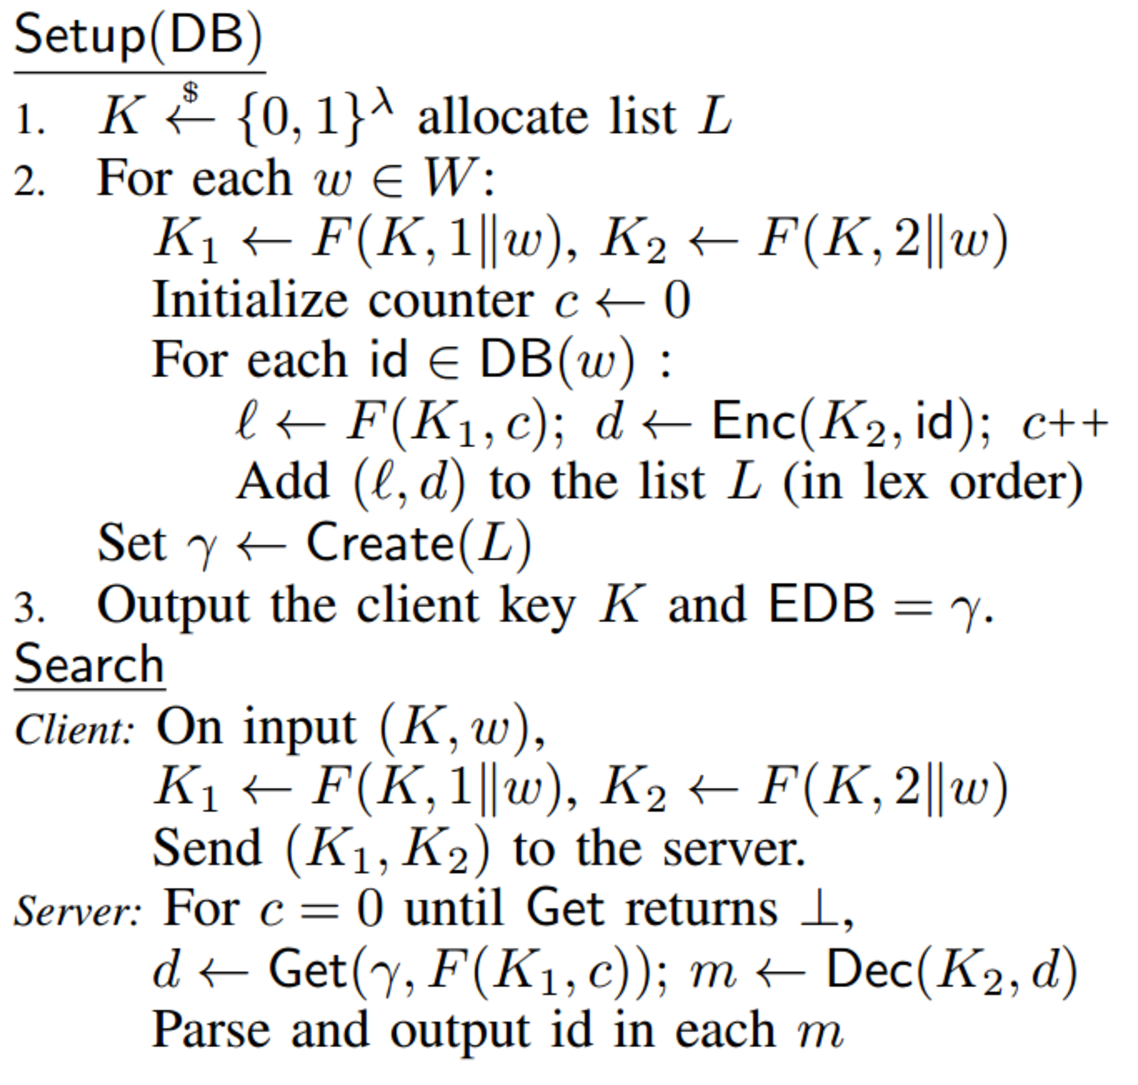
\includegraphics[height=6cm]{PiBaseAlgorithm}
\caption{ $\Pi_{bas}$ algorithm from \cite{davidcashetal.2014}}
\label{fig:pibase-algorithm}
\end{figure}


The search index resulting from $\Pi_{bas}$ is a large number of label/ID pairs. This is somewhat problematic when the goal is to create a practical indexing solution, because of the data size of the index output from this algorithm. The number of pairs ends up being the sum of the number of unique words in each document, summing over all documents, $\sum_{i=0}^{N} |DB(w_i)|$. Beyond SetupDB, searching on the index generated by $\Pi_{bas}$ also has inefficiencies. In order to search for all documents that contain $w$, the search client must execute $|DB(w)|$ independent retrievals. Each retrieval is done with independent keys that have no relation to each other (since they are encrypted), so they won$'$t be grouped together on disk or in memory.

\subsection{Improving Upon $\Pi_{bas}$}
Three modified schemes were introduced that improve upon $\Pi_{bas}$. The first variation after $\Pi_{bas}$ is $\Pi_{pack}$. It uses a very similar approach, but instead of creating each pair of an individual label and document ID, document IDs are grouped in predefined group sizes, with the group size denoted as $B$. Each group of $B$ document IDs are paired with their label. Of course, many of the groups will be not filled up, so any ending empty positions in a group gets padded with values that will not be interpreted as valid document IDs. Keeping a consistent group size is important for security. The importance of this is that the resulting encrypted groups are all the same size. By grouping document IDs in this way, the index that gets built ends up taking up much less space than $\Pi_{bas}$ in practice. A further analysis of this with measurements is included in the implementation section. In addition to a smaller index size, the number of individual searches decrease from $|DB(w)|$ to $\lceil|DB(w)|/B\rceil$.

Further improvements are introduced beyond $\Pi_{pack}$, but their implementations add a new level of implementation complexity beyond the much simpler $\Pi_{bas}$ and $\Pi_{pack}$ schemes. The schemes, $\Pi_{ptr}$ and $\Pi_{2lev}$ may have a much more drastic performance improvement if the search index is stored on disk, which was the case for the experiments run in \cite{davidcashetal.2014}. The improvements involve storing groups of document IDs in memory and in random locations, encrypting pointers to the memory locations, then putting those encrypted pointers into pairs with the labels. In this approach, when a client executes a single search through an on-disk index, they can retrieve $B$ pointers, and use those to retrieve up to $B^2$ documents from memory, faster than they would be retrieved in $\Pi_{pack}$. I will defer to \cite{davidcashetal.2014} for a more in-depth description of these advanced schemes, but due to the specific use of pointers to an in-memory collection of document IDs, the implementation does not fit as nicely into Spark, since the approach would be less efficient if a pointer had to point to a document group on a another node.

\section{IMPLEMENTATION}
This project involved implementing the $\Pi_{bas}$ algorithm, followed by $\Pi_{pack}$. Both are based on an inverted index, which fits fairly well as a Spark implementation. I used an HDFS MapFile as the index storage mechanism, which is a convenient library to use, but not necessarily the most efficient option possible. It stores data in a sorted SequenceFile (which is also an HDFS file format) with its own index to allow for efficient lookups. The MapFile index contains only every 128th key (default setting) so that it can be more easily stored in memory. The implementation in \cite{davidcashetal.2014} uses a dictionary-like structure to store the encrypted index.

\subsection{$\Pi_{bas}$}
Creating an inverted index was the first step towards implementing $\Pi_{bas}$. A common implementation of an inverted index in Spark results in a data structure that contains a map between each word, $w$, and their postings list, which is the unique list of document IDs that the word appears in: $DB(w)$. This was the first step I implemented. The naive approach in Spark is to execute transformations such that you end up with a postings list buffered in memory, and for a large postings list, that may not be scalable. However, getting an entire postings list for a document in memory is not necessary for the $\Pi_{bas}$ scheme, since the goal is to store individual words/docID pairs. The following is a description of the transformations and actions I used in the Spark job for building the index for the $\Pi_{bas}$ algorithm. In hindsight, steps 4 and 5 could have been simpler using a groupBy and map.

\begin{enumerate}
\item flatMap: Parse input file into RDD[(word, docId)]
\item repartitionAndSortWithinPartitions: Group words together by sorting and partitioning using a hash partitioner on the word as the key.
\item mapPartitions: Iterate through each partition. Calculate encrypted labels. Maintain a count, used in the label generation, that gets reset for every new word encountered. Output RDD[(label, (word, docID))]. The word included in the output in order to detect collisions in generated labels.
\item repartitionAndSortWithinPartitions: Sort by encrypted label.
\item mapPartitions: Iterate through labels and determine if there are two of the same labels that correspond to different unencrypted words. If so, this is a collision.
\item sortByKey: Sort must occur prior to saving as MapFile
\item saveAsNewAPIHadoopFile: Save index as MapFile
\end{enumerate}

This approach was not very efficient, though I didn$'$t do any extensive performance testing on it. The index size was very large; even larger than the data size in the example I tested, so rather than well on optimizing it, I moved onto the $\Pi_{pack}$ implementation.

The search component of $\Pi_{bas}$ was fairly straightforward. When a client executes a search for a word, the search algorithm begins a loop with a count that increments with every iteration. The count is used along with the PRF to generate a label for the search word. That label must be the same series of bytes as the label that was generated during the index building stage. The loop exits when no document is found for the generated label. In the case that the search word doesn$'$t exist in any documents, no document ID should be returned in the first iteration of the loop. If the word appears in $n$ documents, iteration $n+1$ should not find a key.

\subsection{$\Pi_{pack}$}
There are various ways in which $\Pi_{pack}$ can be implemented in Spark. The improvement beyond $\Pi_{bas}$ is gained by grouping document IDs into fixed group sizes. If a group size is statically set upfront, the code may be a little bit simpler and more efficient, but in order to experiment with different group sizes, I allowed for the group size to be passed into the Spark job as a parameter. One of the difficulties of this implementation was determining how to group document IDs in to set group sizes of $B$ for a label. A reduceByKey cannot accomplish this. To do it, each label was assigned to a group by giving it a count. The count only incremented after every $B$ document IDs for a label, so that there were $\lceil{DB(w)/B \rceil}$ counts for each label. Then, simply reducing by key and concatenating document ID groups resulted in $\lceil{DB(w)/B \rceil}$ groups for each $w$. The nice thing about this approach is that those groups of document IDs already had the count that was needed for the following step of generating the encrypted label. Here is a description of the transformations and actions I used to implement the $\Pi_{pack}$ index-building algorithm in Spark.

\begin{enumerate}
\item flatMap: Parse input file into RDD[(word, docId)]
\item repartitionAndSortWithinPartitions: Group words together by sorting and repartitioning by $hash(w)\%reducers$
\item mapPartitions: Assign a count to each word and output RDD[((word, count), List[docID])], where the list of docIDs contains only one docID to facilitate a reduce in the next step.
\item reduceByKey: Combing postings lists for each key. Keys contain group counts, so this only generates groups of at most $B$ document IDs.
\item map: Generate encrypted labels for words and output RDD[((label, word), List[docID])]
\item Same as $\Pi_{bas}$ steps 4-7
\end{enumerate}

\subsection{Technical Hurdles}
There were some technical hurdles along the way, as there are in any software development process, but this paper will only focus on the algorithmic hurdles that had to be overcome. Not all of the technical challenges were overcome. One remaining challenge is how to deal with collisions in labels that are generated using the PRF, $F$. These labels need to be random-looking series of bits. In this implementation, they were generated using SHA-256 HMAC, a cryptographic, keyed hash function. Further research is still needed to determine the optimal cryptographic hash function for this purpose, but that is one that is commonly used today for secure network communication.

\section{Results}
\subsection{Environment}
The environment used to run the Spark jobs was a 20-node cluster managed by Altiscale. The cluster had HDFS and Spark installed and configured on it. It was set up as a multi-user environment, but other users had no effect on the measurements taken for the purpose of this project.

\subsection{Datasets}
The concept of a ``document ID'' could represent an actual independent filename or path in this scheme, but in this project, the simplest approach was to use file line offsets within a single HDFS file as document IDs. The requirements of a document ID for this scheme is that it must be a unique value within the document set, and the client must be able to use the document ID to retrieve information from a desired location. If it pointed to a file, then that file could be an encrypted file on a remote server with a file path as a document ID. Servers get to see the document ID for documents retrieved by a query, but that information is commonly leaked by SSE schemes, and there are ways of hiding even that using PIR \cite{davidcashetal.2014}.

The main dataset used for this project was 10\% of English Wikipedia, extracted and loaded into HDFS in the Altiscale environment. It is 1.2 GB on HDFS and is comprised of $\sim$570000 lines, whose file offsets are used as document IDs. A smaller dataset that was used for testing was the ``The Complete Works of William Shakespear'' by project Gutenberg.

\subsection{Index Sizes}
An important performance factor when working towards a practical implementation of an encrypted index is the size of the generated index. $\Pi_{bas}$ ended up generating a larger index than $\Pi_{pack}$, as expected. The index size was much larger than the actual dataset for a small dataset, so I did not run it on the larger 1.2G dataset. When run on the test 5MB dataset, the generated index was 40MB, a factor of 8 times larger. When run on a 188MB dataset containing 1.5\% of English wikipedia, the resulting index was 500MB - a factor of 2.6 times larger.
The $\Pi_{pack}$ approach was run to build the index multiple times, varying the group size each time. The goal with this measurement was to minimize the resulting index size. The breakdown of index sizes is shown in Table \ref{index-sizes}.

\begin{table*}
\centering
\caption{Size of encrypted index files stored as MapFiles on HDFS (MB)}
\label{index-sizes}
\begin{tabular}{|l|l|l|l|} \hline
Group Size & Shakespeare (5MB) & 1.5\% Wiki EN (188MB) & 10\% Wiki EN (1243 MB) \\ \hline
1          & 43.8               & 539                   & --                      \\ \hline
4          & 17                  & 192                    & 1682                \\ \hline
6          & 14.4               & 159                   & 1423                 \\ \hline
8          & 11.8               & 144                   & 1313                 \\ \hline
12         & \textbf{12.6}  & 131                  & \textbf{1241}      \\ \hline
16         & \textbf{12.6}  & \textbf{128}      & 1244                  \\ \hline
24         & 13.5              & 130                  & 1324                  \\ \hline
32         & 14.7              & 135                  & 1443                  \\ \hline
\end{tabular}
\end{table*}

In the datasets measured, there was a clear pattern in the index size relative to the chosen group size. Further measurements could be done to narrow in on a more precise optimal group size for minimizing the index size, but the measurements taken here give a rough idea. The minimum index size for the Shakespeare dataset was around 8 (between 6 and 12). For 1.5\% of English Wikipedia, the minimum index size was found for groups of 16 (between 12 and 24). For 10\% of Wikipedia, the minimum was found for groups of 12 (between 8 and 16).

\subsection{Hash Collisions}
Many encrypted labels are generated in $\Pi_{pack}$. These encrypted labels are random-looking series of bytes, and are of a fixed length. The encrypted label length used in this project was 256 bits, because that$'$s the output of the SHA-256 HMAC algorithm. Like any hash function, there is a certain probability that this will generate collisions. The Spark jobs measured collisions by grouping by labels after they were created, and seeing how many unencrypted words there were for each label. In a complete solution, either encrypted labels would be unique, or there would be a mechanism for dealing with non-unique labels.

In the implementation by Cash et al., they discuss dealing with hash collisions in various ways. One way is using a cuckoo hash. This was determined to save space in \cite{davidcashetal.2014}, where a hash table was used as the index, because they were able to achieve a load of ~90\% in the index hash table, compared to ~60\% using a bucket hash. Rather than deal with collisions in this project, the Spark job detected them and logged them, so that they could be found and counted in the log files generated by the job. They were calculated for the indexes built on the 10\% English Wikipedia dataset. The number of collisions were much higher in the group size of 4 compared to 12 and 24, as shown in Table \ref{hash-collisions}. It is expected that the probability of collisions declines with an increasing group size, because an increase in group size is related to a decrease in the number of encrypted labels that have to be generated.

\begin{table}[]
\centering
\caption{Hash collisions in encrypted labels}
\label{hash-collisions}
\begin{tabular}{ll}
\hline
Group size & Hash Collisions \\ \hline
4          & 14191           \\
12         & 12672           \\
24         & 12440           \\ \hline
\end{tabular}
\end{table}

\section{FUTURE IMPROVEMENTS}
\subsection{Extended Query Capabilities}
Other forms of SSE focus on extending query functionality, and multi-reader/multi-writer capabilities. The form of SSE in this project could be extended to support more than single-word boolean retrieval. The authors of the work in \cite{davidcashetal.2014} investigate this in other works, \cite{jarecki.2013} and \cite{davidcashetal.2013}. In \cite{jarecki.2013}, Cash et al. introduce an OXT (oblivious cross-tags), which is extended by S. Jarecki et al. in \cite{davidcashetal.2013} to support multi-user SSE settings.

The current implementation in this project stores postings lists of document IDs. The document IDs could be replaced with more complex data structures that contain things like exact document locations in which the word occurs, as well as the number of times the word occurs in the document.

\subsection{Postings Compression}
There are some fairly obvious improvements that could be made to the Spark implementation of the index building algorithm. One is compression of the postings list. This could improve both the index size and the running time. Compression could be done in a way such that each full group does not necessary need $B$ document IDs. Instead, the group size would be a byte array size limit, $n_s$. Let the group be a byte array, $s$. The algorithm to build the index could first build a regular inverted index using gap compression on the postings list. Starting with the inverted index, for each word, iterate through the postings list. Begin popping the compressed document IDs from the postings list, copying them one at a time into $s$. Once $s$ has reached capacity $n_s$, start filling in the next group. This way, you will likely end up with more than $B$ document IDs in each group $s$. The index storage size benefit is obvious, but this would also likely result in less data to shuffle between nodes in the Spark environment, which could lead to an improvement in running time of the index building job. If group sizes are larger, the the client has to execute fewer individual retrievals on average, so search efficiency could also improve.

\begin{enumerate}
\item flatMap: Parse input file into RDD[(word, docId)]
\item repartitionAndSortWithinPartitions: Order words together by sorting and partitioning using \\
$hash(w)\%reducers$

\item mapPartitions: Iterate through each partition. Build compressed postings lists for each word. Reset postings list when encountering a new word. Outputs \\ RDD[(word, compressedPostings)]

\item flatMap: Iterate through compressedPostings. Copy compressed postings ID into byte array $s$ until it is full. Output that group with the current encrypted label, and create a new group. Each encrypted label is tied to an integer count, so these groups will be ordered upon retrieval (necessary for reversing gap compression).

\item sortByKey: Sort must occur prior to saving as MapFile

\item saveAsNewAPIHadoopFile: Save index as MapFile
\end{enumerate}

\subsection{Hash Collision Resolution}
Hash collisions could be dealt with in a bucket hash manner, but this has potential security issues. A collision is encountered when two encrypted labels are generated that match. The most basic approach would be to use a bucket hash, where the colliding document ID groups are chained or concatenated. Upon searching, the client would have to determine which part of the bucket contained the document ID group that it was searching for. Each group will have been encrypted using a key that incorporates the search word, so one potential option is to include extra data in the document ID groups so that the client can determine when they$'$ve found the correct group. They should only be able to properly decrypt the group for the word they are searching on. The extra information should be included prior to encrypting the postings lists rather than appended onto the already encrypted groups, otherwise the added information will be leaked.

\subsection{Security}
This project had very little focus on security. It is assumed that the algorithm implementation didn$'$t change the security proofs described in \cite{davidcashetal.2014} in a way that would leak any more information. The current project implementation did not encrypt postings lists, but it did group document IDs together to get an idea of the resulting index data sizes when postings lists are grouped like in $\Pi_{pack}$. Encrypting the document ID groups should be a trivial extension to the current implementation.

\subsection{Document Updating} 
This project also didn$'$t broach the subject of document updating. In \cite{davidcashetal.2014}, there are variants of dynamic update protocols that work with all the static variants ($\Pi_{bas}$, $\Pi_{pack}$, $\Pi_{ptr}$, $\Pi_{2lev}$). These could be implemented in a Spark job as well, but I will leave that discussion to future research.

\subsection{Performance Tuning}
More performance tuning and optimization for memory-management could be done. A good area of improvement would be the approach used to group document IDs. Group size is passed to the Spark job as an input parameter, but it could be hard-coded to gain some performance advantages. If it were hard-coded, the Spark algorithms to build the index could remove any loops over the document group size. Those parts could then make better use of processor pipelining.

\section{Conclusions}
The $\Pi_{bas}$ and $\Pi_{pack}$ algorithms translated quite fluently into Spark jobs. They were easily parallelizable. 


Searchable encryption is an interesting area of research with interesting applications, anywhere that data privacy is critical. While there has been a lot of progress in SSE research since the pioneering work of Song, Wagner and Perrig in 2000 \cite{swp.2000}, there is still not an obviously practical solution for many uses. Cash et al. showed that indexes can be created on terabyte-scale datasets, but their implementation had some drawbacks, in that it still could take multiple days to generate the index for datasets of this size. Their implementation was run on a large scaled-up server. The underlying performance problem was not solved by the trivial implementation executed in this project, but it was shown that their $\Pi_{bas}$ and $\Pi_{pack}$ algorithm can be be parallelized in a Spark environment, and because of that, it can be scaled horizontally. 

A potential use for an encrypted index is that a client could build their encrypted index locally and upload it to a remote server, then still be able to search on it. Trust concerns between client and server would diminish, since the remote server could not interpret the uploaded data. If a client has to put the data into a Spark environment to create the encrypted index in the first place, new trust issues arise between the client and the distributed Spark systems. If a client can$'$t trust a remote storage server, then building the index in a distributed system like Spark may not be acceptable for that use case. This use case could still be acceptable if the Spark environment is within a trusted firewall, but a storage server is outside the firewall.

A comparison to the approach by Cash et al would be interesting with more performance measurements and by running the algorithms on a similar dataset size. Future work can build off of this initial project to really test the waters of how practical these SSE schemes can be when run on terabyte-scale datasets and beyond, especially if they can make use of commodity hardware and horizontal scaling.



% Bibliography %
% ============ %
\bibliographystyle{abbrv}
\bibliography{encryptedIndexSpark}

\end{document}